%
% Optical Routers
%

\section{Optical routers} \index{Optical routers}

\dropcap{P}{erhaps} the most fundamental building block in any network is routers, devices which switch data packets between multiple inputs and outputs so as to relay them to a destination. Indeed, in many real-world networks, many nodes will purely implement routing, and nothing more elaborate such as computations or other end-user protocols, to be discussed in Sec.~\ref{sec:protocols_quant_int}.

We now discuss the implementation of optical routers, beginning with the simplest two-port switch, upon which we build to construct more general and powerful routers.

We will use the terminology that:
\begin{itemize}
	\item \textit{Ports}\index{Ports}: refers to the number of input and output optical modes in a device.
	\item \textit{Channels}\index{Channels}: refers to the number of simultaneous communications streams running in parallel through the device.
	\item \textit{Optical depth}\index{Optical depth}: is the number of primitive optical elements/devices an optical path traverses through the course of its trajectory from input to output.
\end{itemize}

A summary of the routing devices we consider, and their associated resource requirements, is provided in Table.~\ref{tab:router_summary}.

Of course, real-world routers will not only switch optical paths, but also implement some (probably undesired) quantum processes across those paths, such as a loss channel or temporal mode-mismatch. Thus, proper analysis of optical router performance in quantum networks requires treating them as legitimate nodes in the network graph, with associated costs and attributes, as per the QTCP framework.

\startnormtable
\begin{table*}[!htbp]
	\begin{tabular}{|c|c|c|}
		\hline
  		Device & Resource requirements & Optical depth \\
  		\hline
  		\hline
  		Two-channel two-port switch & \mbox{$N_\mathrm{bs}=2$}, \mbox{$N_\mathrm{ps}=1$} & \mbox{$d=1$} \\
  		Linear $n$-port multiplexer & \mbox{$N_\mathrm{s}=n-1$} & \mbox{$1\leq d\leq n-1$} \\
  		Pyramid $n$-port multiplexer & \mbox{$N_\mathrm{s}=n-1$} & \mbox{$d=\log_2(n)$} \\
    	Single-channel multi-port switch (linear) & \mbox{$N_\mathrm{s}=2n-3$} & \mbox{$2\leq d\leq 2n-3$} \\
  		Single-channel multi-port switch (pyramid) & \mbox{$N_\mathrm{s}=2n-3$} & \mbox{$d=2\,\log_2(n)-1$} \\
  		Multi-channel multi-port switch & \mbox{$N_\mathrm{s} = \left\lceil \frac{n^2}{2}\right\rceil - n + 1$} & \mbox{$\left\lceil \frac{n}{2} \right\rceil \leq d\leq n-1$} \\
  		Crossbar switch & \mbox{$N_\mathrm{s}=n^2$} & \mbox{$1\leq d\leq 2n-1$}\\
    	\hline
	\end{tabular}
	\captionspacetab \caption{Summary of different primitives for constructing optical routers. $n$, $N_\mathrm{bs}$, $N_\mathrm{ps}$ and $N_\mathrm{s}$ are the number of input/output ports, beamsplitters, phase-shifters, and two-port switches respectively. $d$ is the optical depth (in units of number of two-port switches). Since all of the multi-port devices are constructed from two-port switches, in all cases \mbox{$N_\mathrm{bs} = 2 N_\mathrm{s}$} and \mbox{$N_\mathrm{ps} = N_\mathrm{s}$}.} \label{tab:router_summary} \index{Optical routers}\index{Optical depth}\index{Router resource requirements}
\end{table*}
\startalgtable

%
% Mechanical Switches
%

\subsection{Mechanical switches}\index{Mechanical switches}

Most obviously, optical switching could be performed mechanically, by physically displacing fibre endpoints, directing them towards different routes\footnote{Remember, the telephone network used to be mechanically routed by human switchboard operators, manually routing point-to-point connections!}. Such switches have found use in other areas, but are not particularly appropriate for quantum information processing applications, as they are extremely slow compared to electro- or acousto-optic technologies. Certainly, mechanical switching would not be applicable to optical fast-feedforward, such as that required by optical quantum computing, on the order of nanoseconds.

A second disadvantage of mechanical switches is that the introduction of moving parts into quantum optics protocols makes optical stabilisation extremely challenging. The mechanical control required to preserve wavelength-level coherence, for example, is effectively ruled out by moving mechanical parts.

%
% Interferometric Routers
%

\subsection{Interferometric routers} \index{Interferometric routers}

Interferometric routers are based on the principle that the evolution implemented by interferometers are in general highly dependent on the phase relationships within them. This reduces the seemingly uphill task of high-speed, dynamic switching between modes to the problem of implementing dynamically-controllable phases. Thankfully there are a number of techniques for implementing such phase-switching. We will discuss these phase-modulation techniques, before moving onto combining them into more complex routing systems.

%
% Phase-Modulators
%

\subsubsection{Phase-modulators} \index{Phase-modulators}

A phase-modulator is a classically-controlled device that lets us tune the local phase accumulated by an optical path, ideally over the full range of $\{0,2\pi\}$. These may be implemented in several ways:

\comment{Rohit helps here}

%
% Electro-Optic Modulators
%

\paragraph{Electro-optic modulators} \index{Electro-optic modulators}

\comment{here an applied electric field induces a change in refractive index in a medium, causing a phase-shift.}

\comment{To do! Explain how these work}

%
% Acousto-Optic Modulators
%

\paragraph{Acousto-optic modulators} \index{Acousto-optic modulators}

\comment{an applied acoustic wave generated by a piezoelectric transducer induces a change in refractive index in a medium, causing a phase-shift}

\comment{To do! Explain how these work}

%
% Magneto-Optic Modulators
%

\paragraph{Magneto-optic modulators} \index{Magneto-optic modulators}

\comment{an applied magnetic field induces the change in refractive index}

\comment{To do! Explain how these work}

%
% Pockels Cells
%

\paragraph{Pockels cells} \index{Pockels cells}

\comment{act as voltage-controlled wave-plates, 	which take the place of phase-shifters in a polarisation-encoded version of Mach-Zehnder interference.}

\comment{To do! Explain how these work}

%
% Two-Channel Two-Port Switches
%

\subsubsection{Two-channel two-port switches} \index{Two-channel two-port switches}

The elementary primitive switch from which more complicated routers may be constructed is the two-channel two-port switch. This switch may be constructed from a Mach-Zehnder interferometer\index{Mach-Zehnder (MZ) interference}, with a classically-controlled phase-shifter in one arm. By switching the phase to either \mbox{$\phi=0$} or \mbox{$\phi=\pi$}, the MZ may be tuned to implement either an identity or swap operation respectively. This is shown in Fig.~\ref{fig:two_channel_two_port_switch}.

In the upcoming diagrams we present, arrows are used to indicate the time-ordering of the flow of data. However, it should be noted that a MZ interferometer is reversible and therefore bidirectional, and so too are all of the more complex routers based upon them.

\begin{figure}[!htbp]
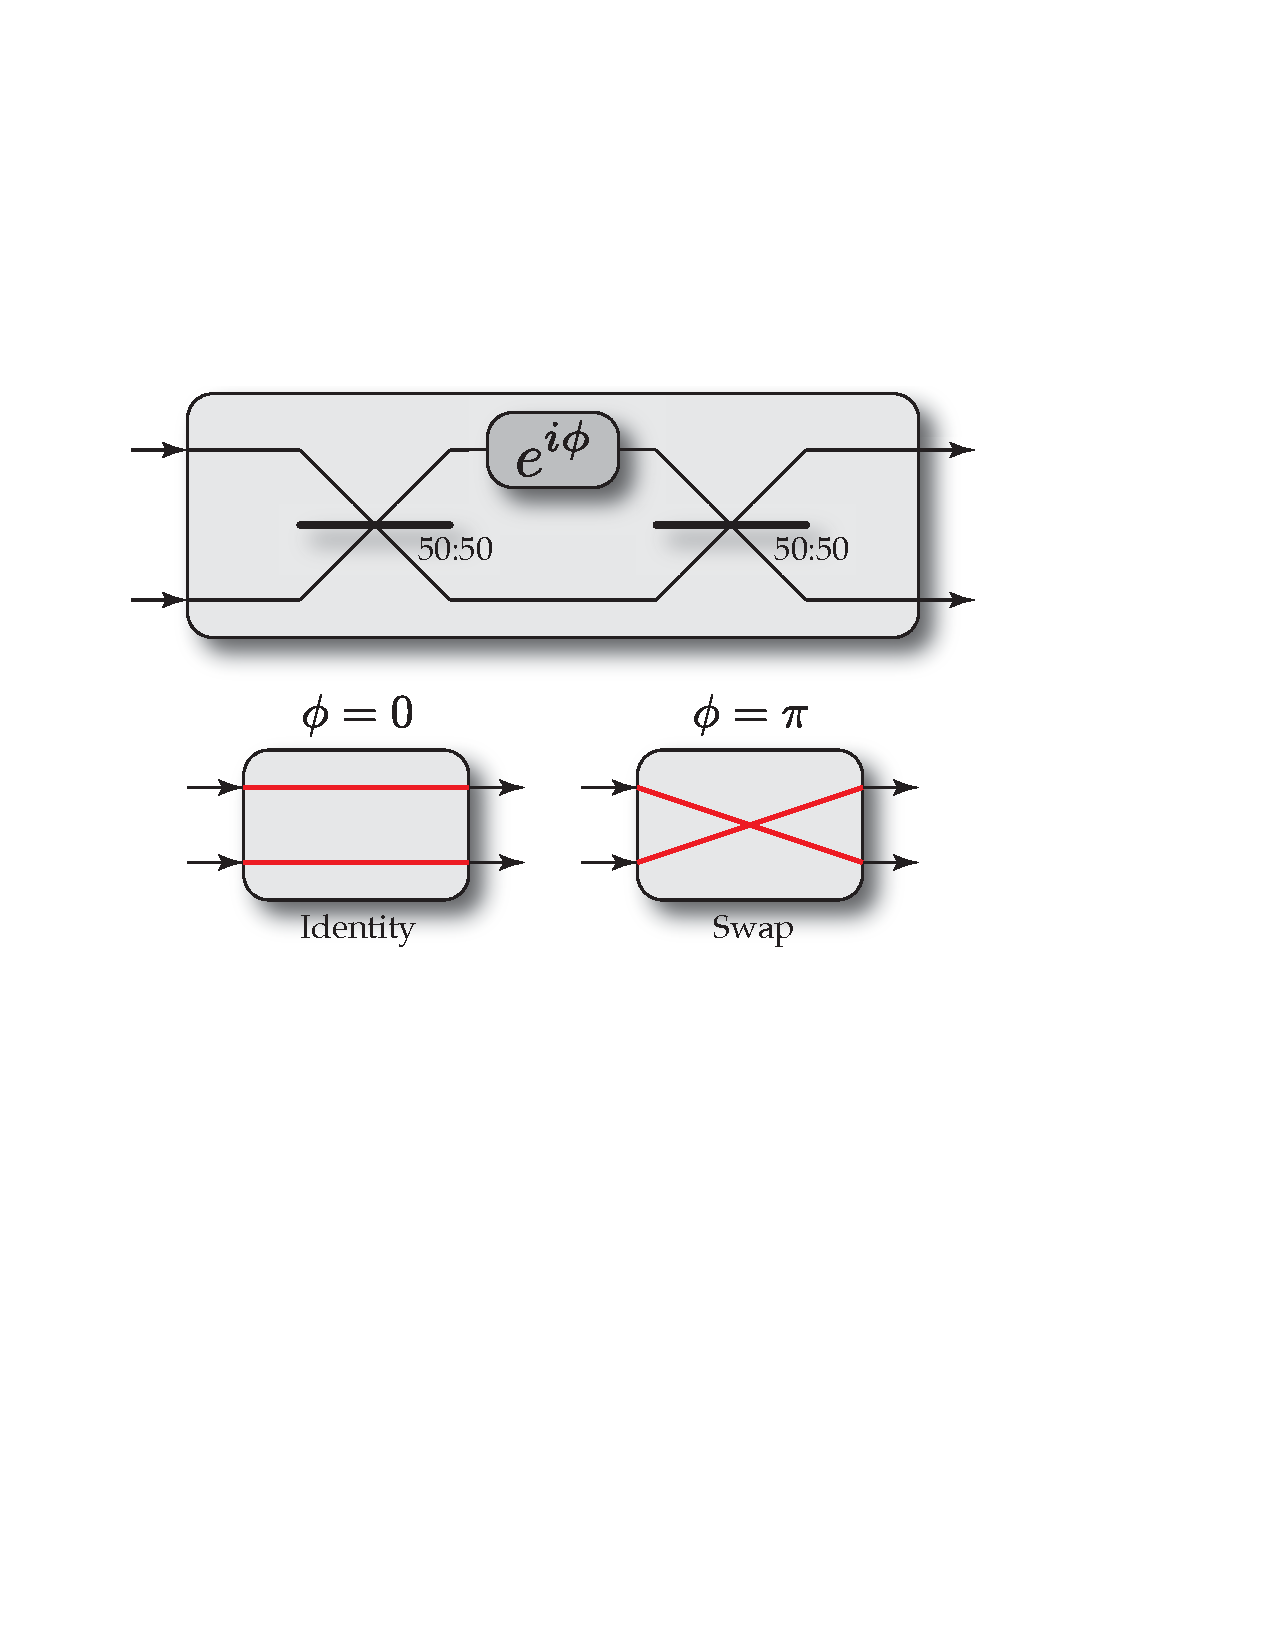
\includegraphics[clip=true, width=0.475\textwidth]{two_channel_two_port_switch}
\captionspacefig \caption{(top) A two-channel two-port switch has two inputs and two outputs, implementing either an identity or swap operation between them. This may be constructed using a Mach-Zehnder interferometer with a variable, classically-controlled phase-shift, $e^{i\phi}$, in one of the arms, which may be implemented using an acousto-optic or electro-optic modulator (AOM or EOM). The phase-shift is allowed to be either \mbox{$\phi=0$} for an identity channel (bottom left) or \mbox{$\phi=\pi$} for a swap operation (bottom right). Because the switch is based on MZ interference, this technique only applies to optical states which undergo MZ interference. The total resource requirements are two 50:50 beamsplitters and a single phase-shifter.} \label{fig:two_channel_two_port_switch} \index{Two-channel two-port switches}\index{Mach-Zehnder (MZ) interference}
\end{figure}

Because the two-port switch is based upon MZ interference, it will only function for optical states subject to such MZ interference. Thus, single-photons and coherent states are applicable, whereas thermal states, for example, are not.

%
% Multiplexers & Demultiplexers
%

\subsubsection{Multiplexers \& demultiplexers} \index{Multiplexers}\index{Demultiplexers}

From the two-port switch, which implements a controlled permutation of two optical modes, we can construct multi-port multiplexers and demultiplexers, which controllably route a single input port to one of $n$ multiple output ports, or vice versa.

There are two main architectures that may be employed for implementing such multiplexers/demultiplexers. The first is to use a linear cascade of two-port switches, shown in Fig.~\ref{fig:linear_multiplexer}\index{Linear multiplexers \& demultiplexers}. The second is to use a pyramid cascade, shown in Fig.~\ref{fig:pyramid_multiplexer}\index{Pyramid multiplexers \& demultiplexers}. Both layouts require,
\begin{align}
N_\mathrm{s} = n-1,
\end{align}
two-port switches to implement. However, they differ in one important respect. In the linear multiplexer, different routes experience different optical depth\index{Optical depth}, ranging from \mbox{$d=1$} (for the first port) to \mbox{$d=n-1$} (for the final port). This will lead to asymmetry in accumulated errors. In the pyramid multiplexer, on the other hand, all optical paths have the same optical depth, \mbox{$d=\log_2(n)$}, yielding completely symmetric operation.

The differing optical depths of linear and pyramid multiplexers lend themselves naturally to different applications. Suppose that in a network a single input-to-output route through a multiplexer is used far more often than the others. In that case, utilising a linear multiplexer will minimise average optical depth since that route can be designated to the first output port, which has an optical depth of only \mbox{$d=1$}. On the other hand, in a very balanced network, in which all optical routes are used roughly uniformly, the average case logarithmic optical depth of the pyramid multiplexer outperforms the average case linear optical depth of the linear multiplexer.

Note that the logarithmic optical depth of the pyramid configuration grows less quickly than the linear average optical depth of the linear configuration. Thus, on average, optical paths pass through fewer optical elements in the pyramid configuration, reducing average accumulated error rates when using noisy optical elements. This, in conjunction with the pyramid's perfect symmetry, makes the pyramid multiplexer configuration generally most favourable.

\begin{figure}[!htbp]
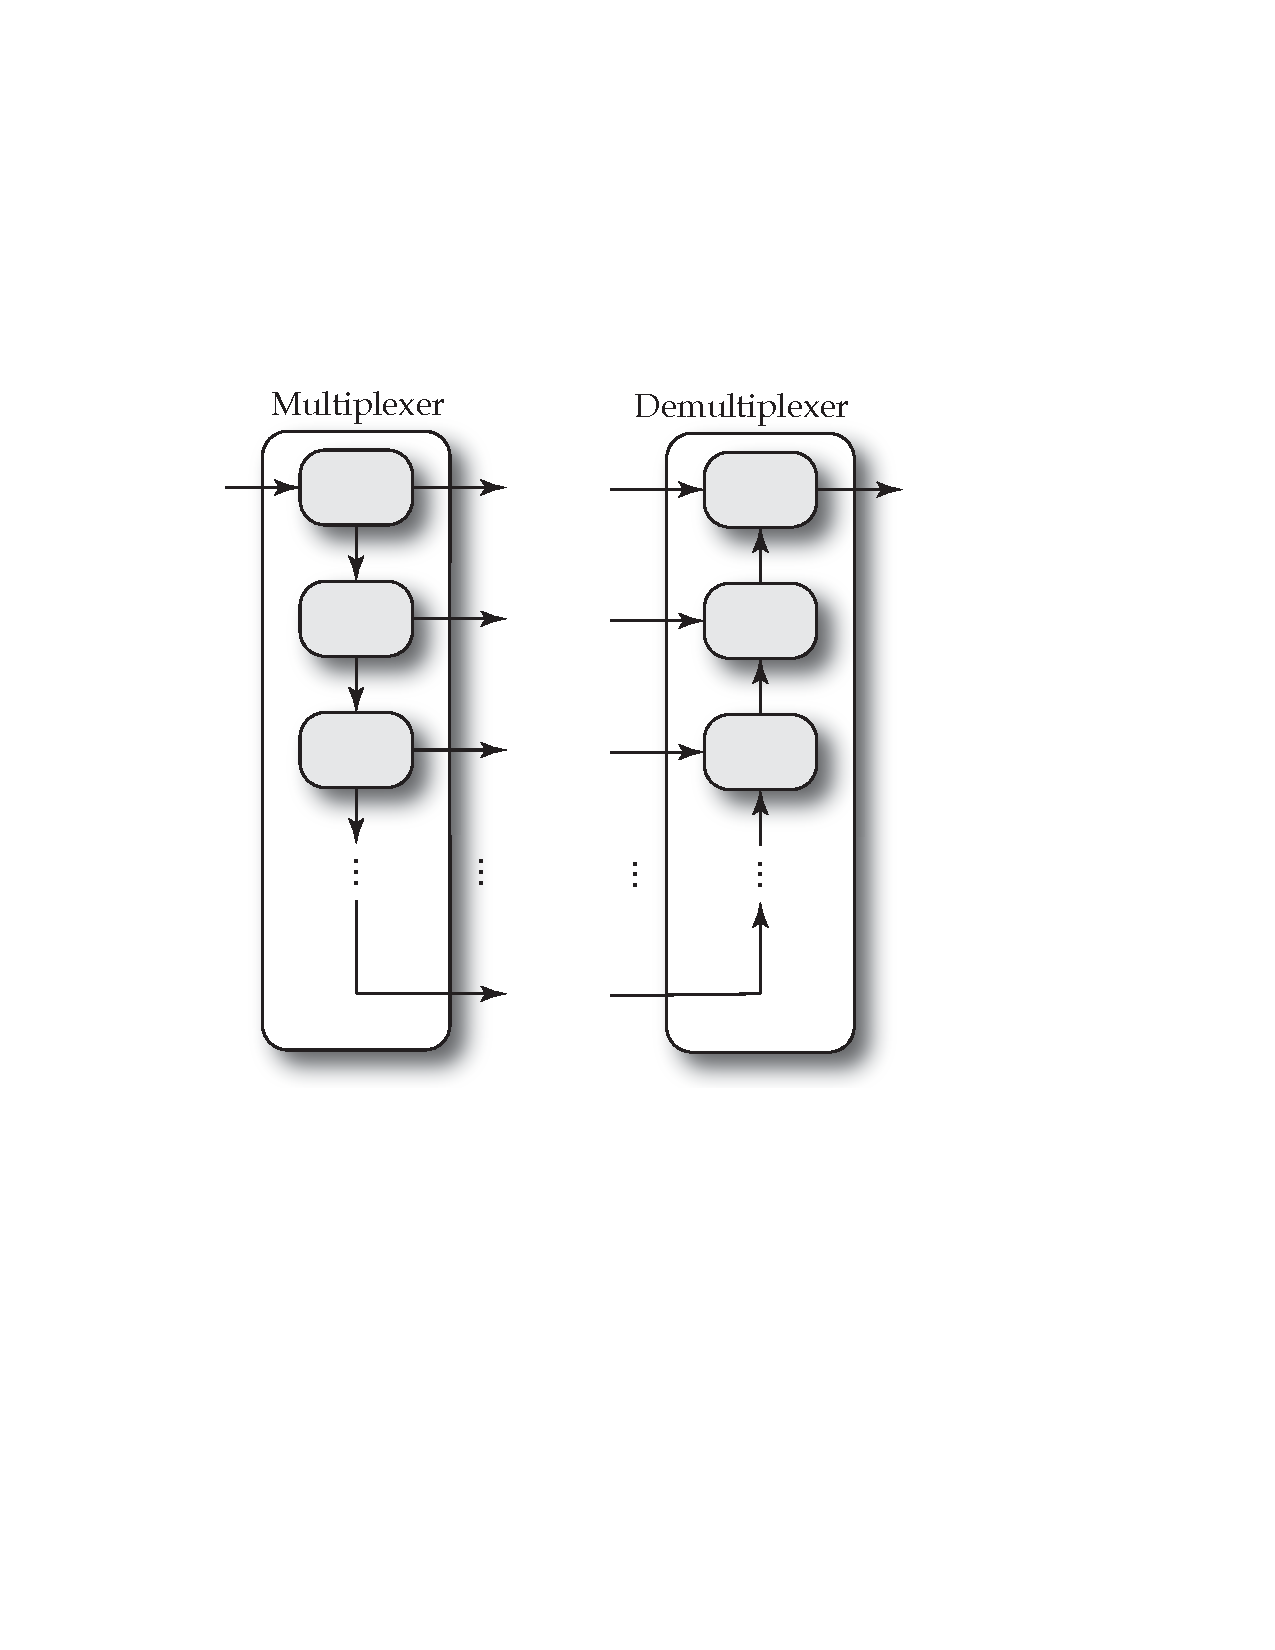
\includegraphics[clip=true, width=0.425\textwidth]{linear_multiplexer}
\captionspacefig \caption{Linear multiplexers (left) and demultiplexers (right) may be constructed from a linear chain of two-port switches (grey boxes), cascading into one another. These switch a single optical channel between $n$ ports. The total resource requirements are \mbox{$n-1$} two-port switches. The optical depth ranges from $1$ (for the first port) to \mbox{$n-1$} (for the final port).} \label{fig:linear_multiplexer} \index{Linear multiplexers \& demultiplexers}
\end{figure}

\begin{figure}[!htbp]
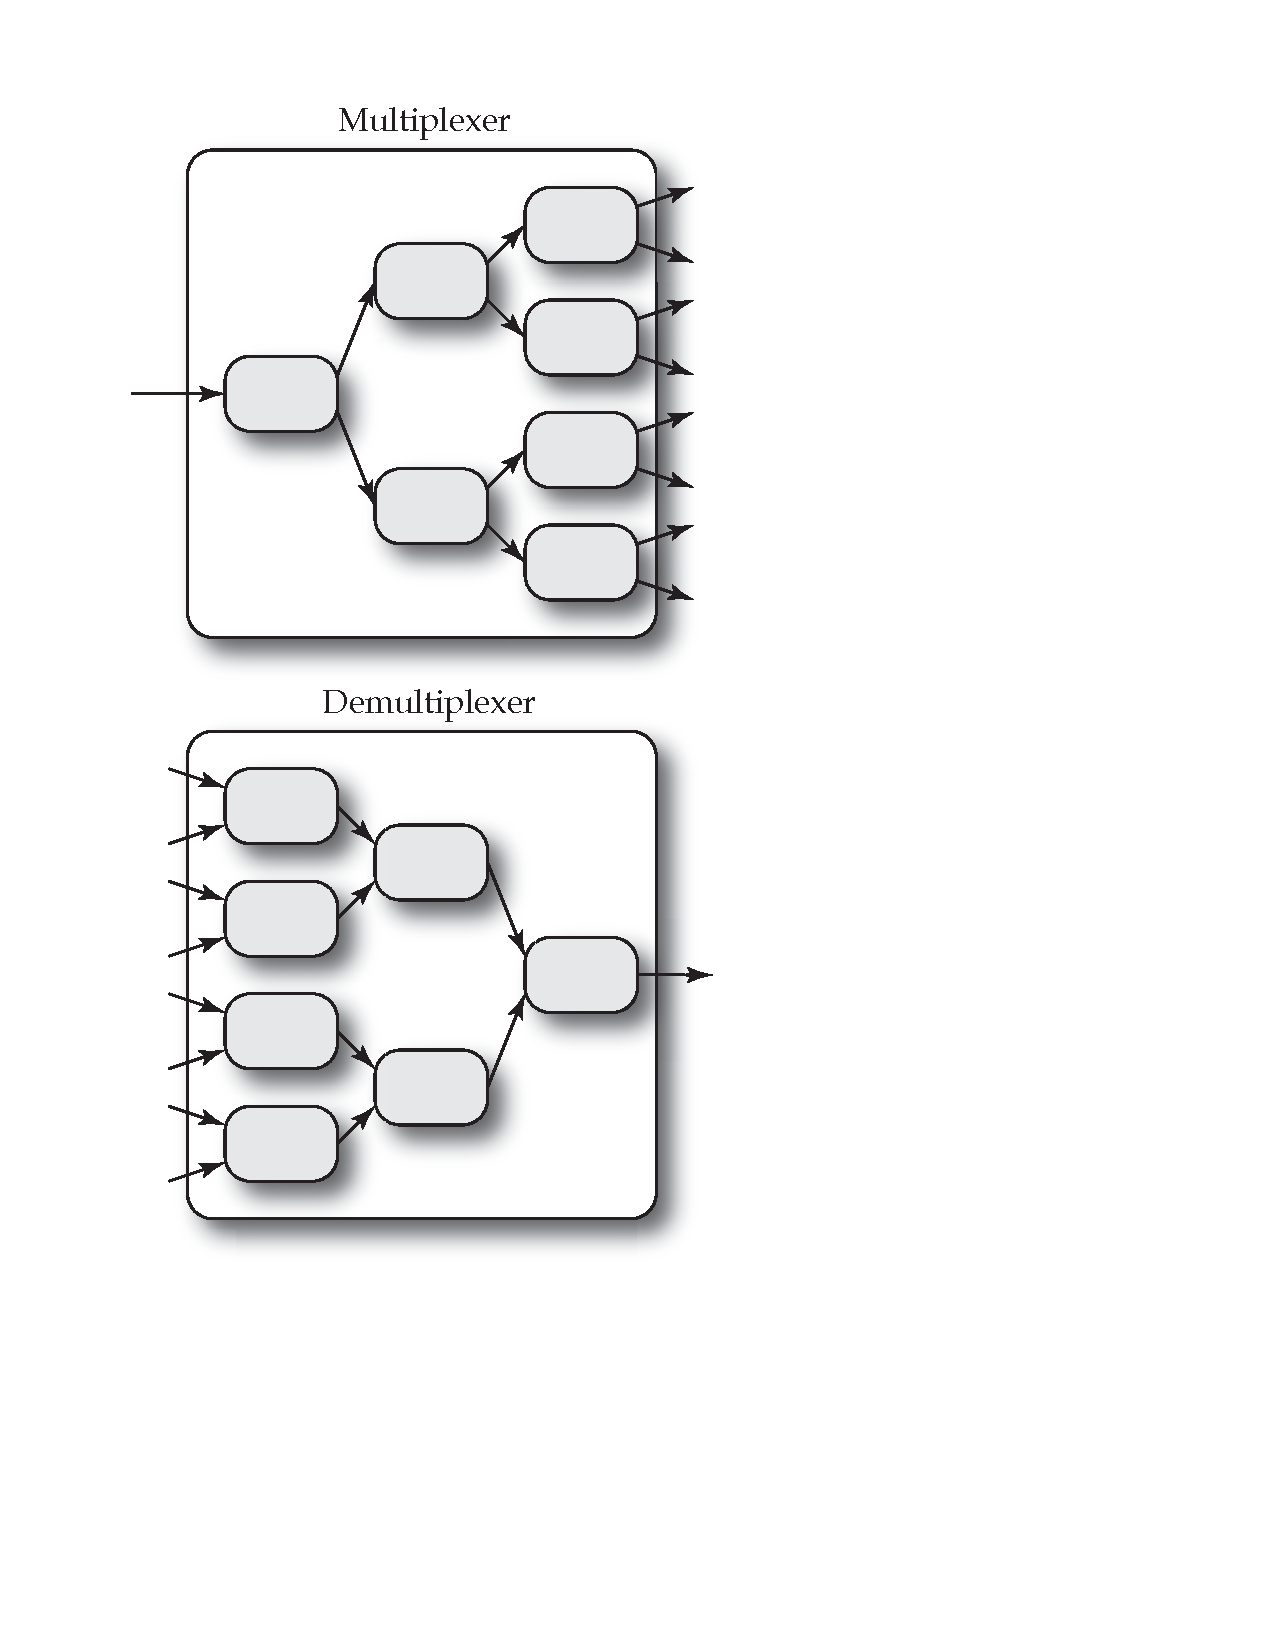
\includegraphics[clip=true, width=0.35\textwidth]{pyramid_multiplexer}
\captionspacefig \caption{Pyramid multiplexers (top) and demultiplexers (bottom) decompose the multiplexing into a binary tree-structure of two-port switches (grey boxes), shown here for the case of \mbox{$n=8$} ports. For $n$ ports, all optical paths observe an optical depth of \mbox{$d=\log_2(n)$} two-port switches, of which there are \mbox{$n-1$} in total.} \label{fig:pyramid_multiplexer} \index{Pyramid multiplexers \& demultiplexers}
\end{figure}

%
% Single-Channel Multi-Port Switches
%

\subsubsection{Single-channel multi-port switches} \index{Single-channel multi-port switches}

The multiplexers and demultiplexers route between one port and $n$ ports. In the more general and useful case, we wish to route between $n$ inputs and $n$ outputs. If we only require one active channel at a given time, such a router may be trivially constructed from an $n$-port multiplexer connected to and $n$-port demultiplexer, as shown in Fig.~\ref{fig:single_channel_multi_port_switch}. Here the demultiplexer chooses one of the input modes to route to its single output, which then feeds into the multiplexer to fan it out to the desired output. The multiplexers/demultiplexers could be implemented using either of the aforementioned layouts, yielding a total resource count of,
\begin{align}
	N_\mathrm{s} = 2n-3,
\end{align}
two-port switches\footnote{Note that the multiplexer and demultiplexer each require \mbox{$2(n-1)$} two-port switches, but one of the central ones adjoining the multiplexer and demultiplexer is redundant and may be eliminated, reducing the number of two-port switches to \mbox{$2n-3$}.}.

\begin{figure}[!htbp]
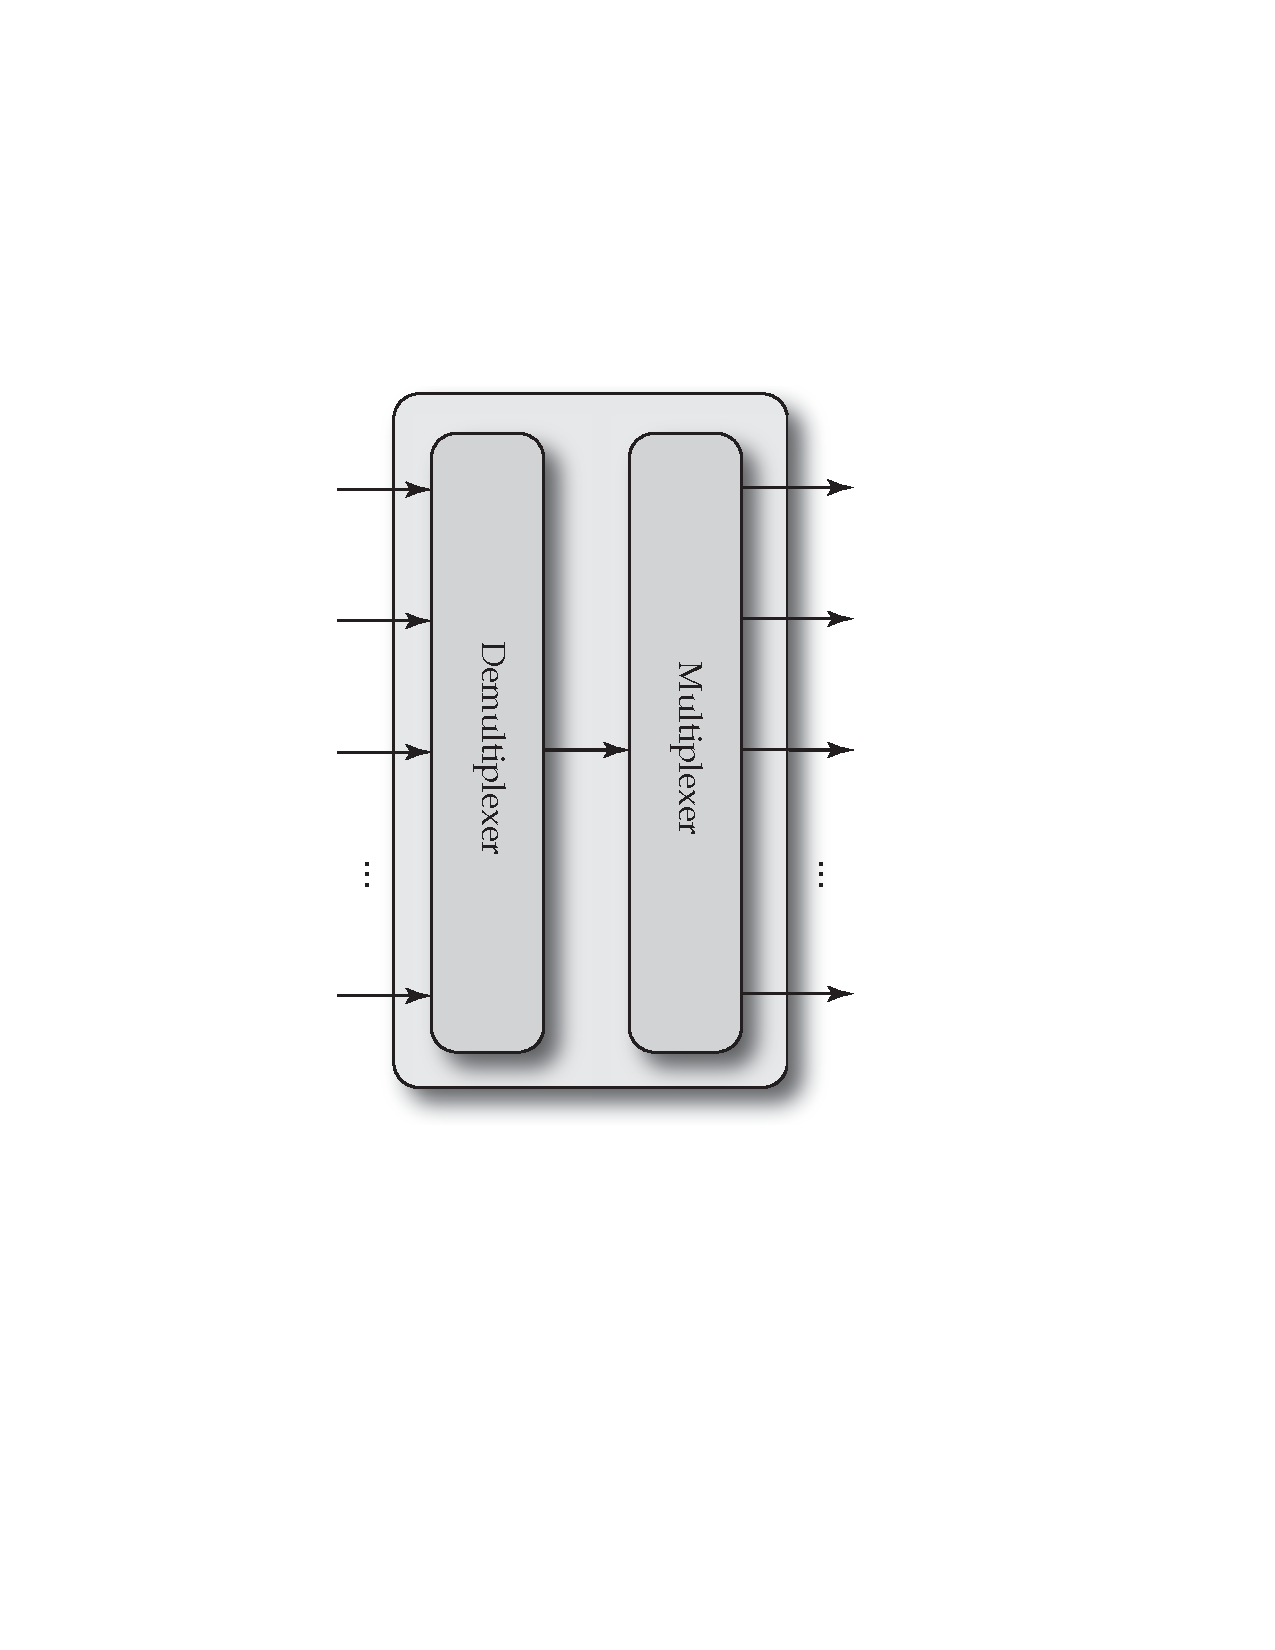
\includegraphics[clip=true, width=0.375\textwidth]{single_channel_multi_port_switch}
\captionspacefig \caption{A single-channel multi-port switch may be constructed by demultiplexing the $n$ input ports to a single port, routing the desired input channel to that port, before multiplexing it back out to the desired output port. This allows an arbitrary input to be routed to an arbitrary output, but only one channel at a time. This requires \mbox{$2n-3$} two-port switches in total.} \label{fig:single_channel_multi_port_switch} \index{Single-channel multi-port switches}	
\end{figure}

%
% Multi-Channel Multi-Port Switches
%

\subsubsection{Multi-channel multi-port switches} \index{Multi-channel multi-port switches}

The single-channel multi-port switch enables switching between an arbitrary number of input/output ports, but suffers that it can only route a single channel at a time. The most general scenario to consider is multi-channel multi-port switching, which implements an arbitrary permutation between $n$ inputs and $n$ outputs. That is, all $n$ ports may be routing active channels, enabling simultaneous routing of multiple data-flows.

Such a switch may be constructed from a staggered, rectangular lattice of two-port switches, as shown in Fig.~\ref{fig:multi_channel_multi_port_switch}. It is easy to see upon inspection that optical paths exist between every input/output pair of ports. The total resource count for this device is,
\begin{align}
N_\mathrm{s} = \left\lceil \frac{n^2}{2}\right\rceil - n + 1,
\end{align}
two-port switches.

The operation implemented by this device can therefore be expressed as,
\begin{align}
	\left(\begin{matrix}{}
  		\hat{b}^\dag_1 \\
  		\hat{b}^\dag_2 \\
  		\vdots \\
  		\hat{b}^\dag_m
\end{matrix}\right)=\sigma\cdot\left(\begin{matrix}{}
  		\hat{a}^\dag_1 \\
  		\hat{a}^\dag_2 \\
  		\vdots \\
  		\hat{a}^\dag_m
\end{matrix}\right),
\end{align}
where \mbox{$\sigma\in S_m$} is an arbitrary element of the symmetric group (i.e a permutation matrix), and $\hat{a}_i^\dag$ ($\hat{b}_i^\dag$) are the input (output) photonic creation operators.

\begin{figure}[!htbp]
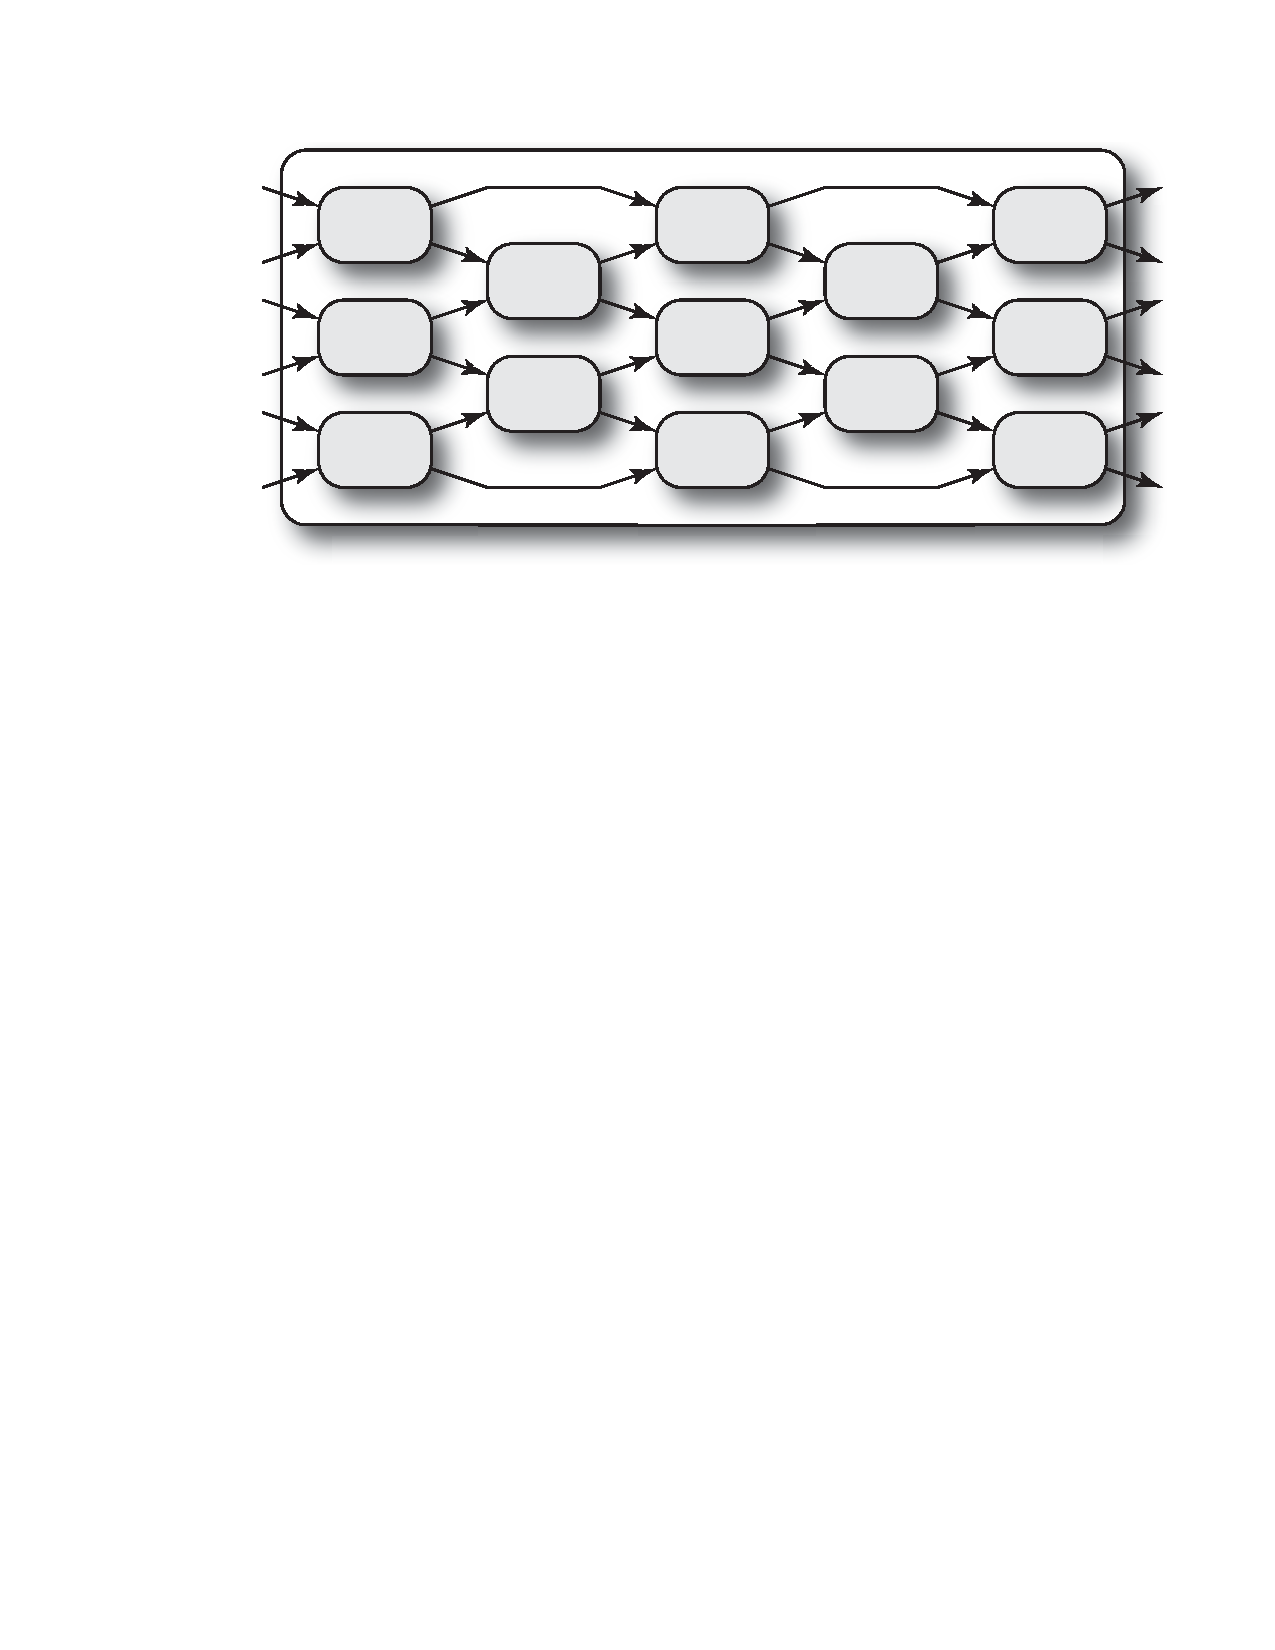
\includegraphics[clip=true, width=0.475\textwidth]{multi_channel_multi_port_switch}
\captionspacefig \caption{A completely general multi-channel multi-port switch may be constructed using a staggered grid of two-port switches (grey boxes), shown here for \mbox{$n=6$} ports. This allows the implementation of an arbitrary permutation between input and output ports, enabling all $n$ channels to be simultaneously utilised and routed across distinct input-to-output routes. This requires \mbox{$\left\lceil \frac{n^2}{2}\right\rceil - n + 1$} two-port switches in total. Optical depth is approximately equal across all input-to-output paths.} \label{fig:multi_channel_multi_port_switch} \index{Multi-channel multi-port switches}	
\end{figure}

Note that this decomposition is more favourable than the completely general Reck \textit{et al.} decomposition presented in Fig.~\ref{fig:LO_archs}(a), since the circuit is balanced, with (almost!) identical optical depths across all input-to-output paths.

%
% Crossbar Switches
%

\subsubsection{Crossbar switches}\index{Crossbar switches}

A general multi-port switching architecture, that gained popularity in the early days of channel-switched telecommunications networks\index{Channel-switched networks}, is the crossbar architecture, whereby $n$ inputs are mapped to $n$ outputs via a binary permutation matrix, which controls a lattice of \mbox{$2\times 2$} switches. The general layout of the architecture is shown in Fig.~\ref{fig:crossbar_switch}, and an example of a routing sequence corresponding to a particular binary control matrix is shown in Fig.~\ref{fig:crossbar_example}.

\begin{figure}[!htbp]
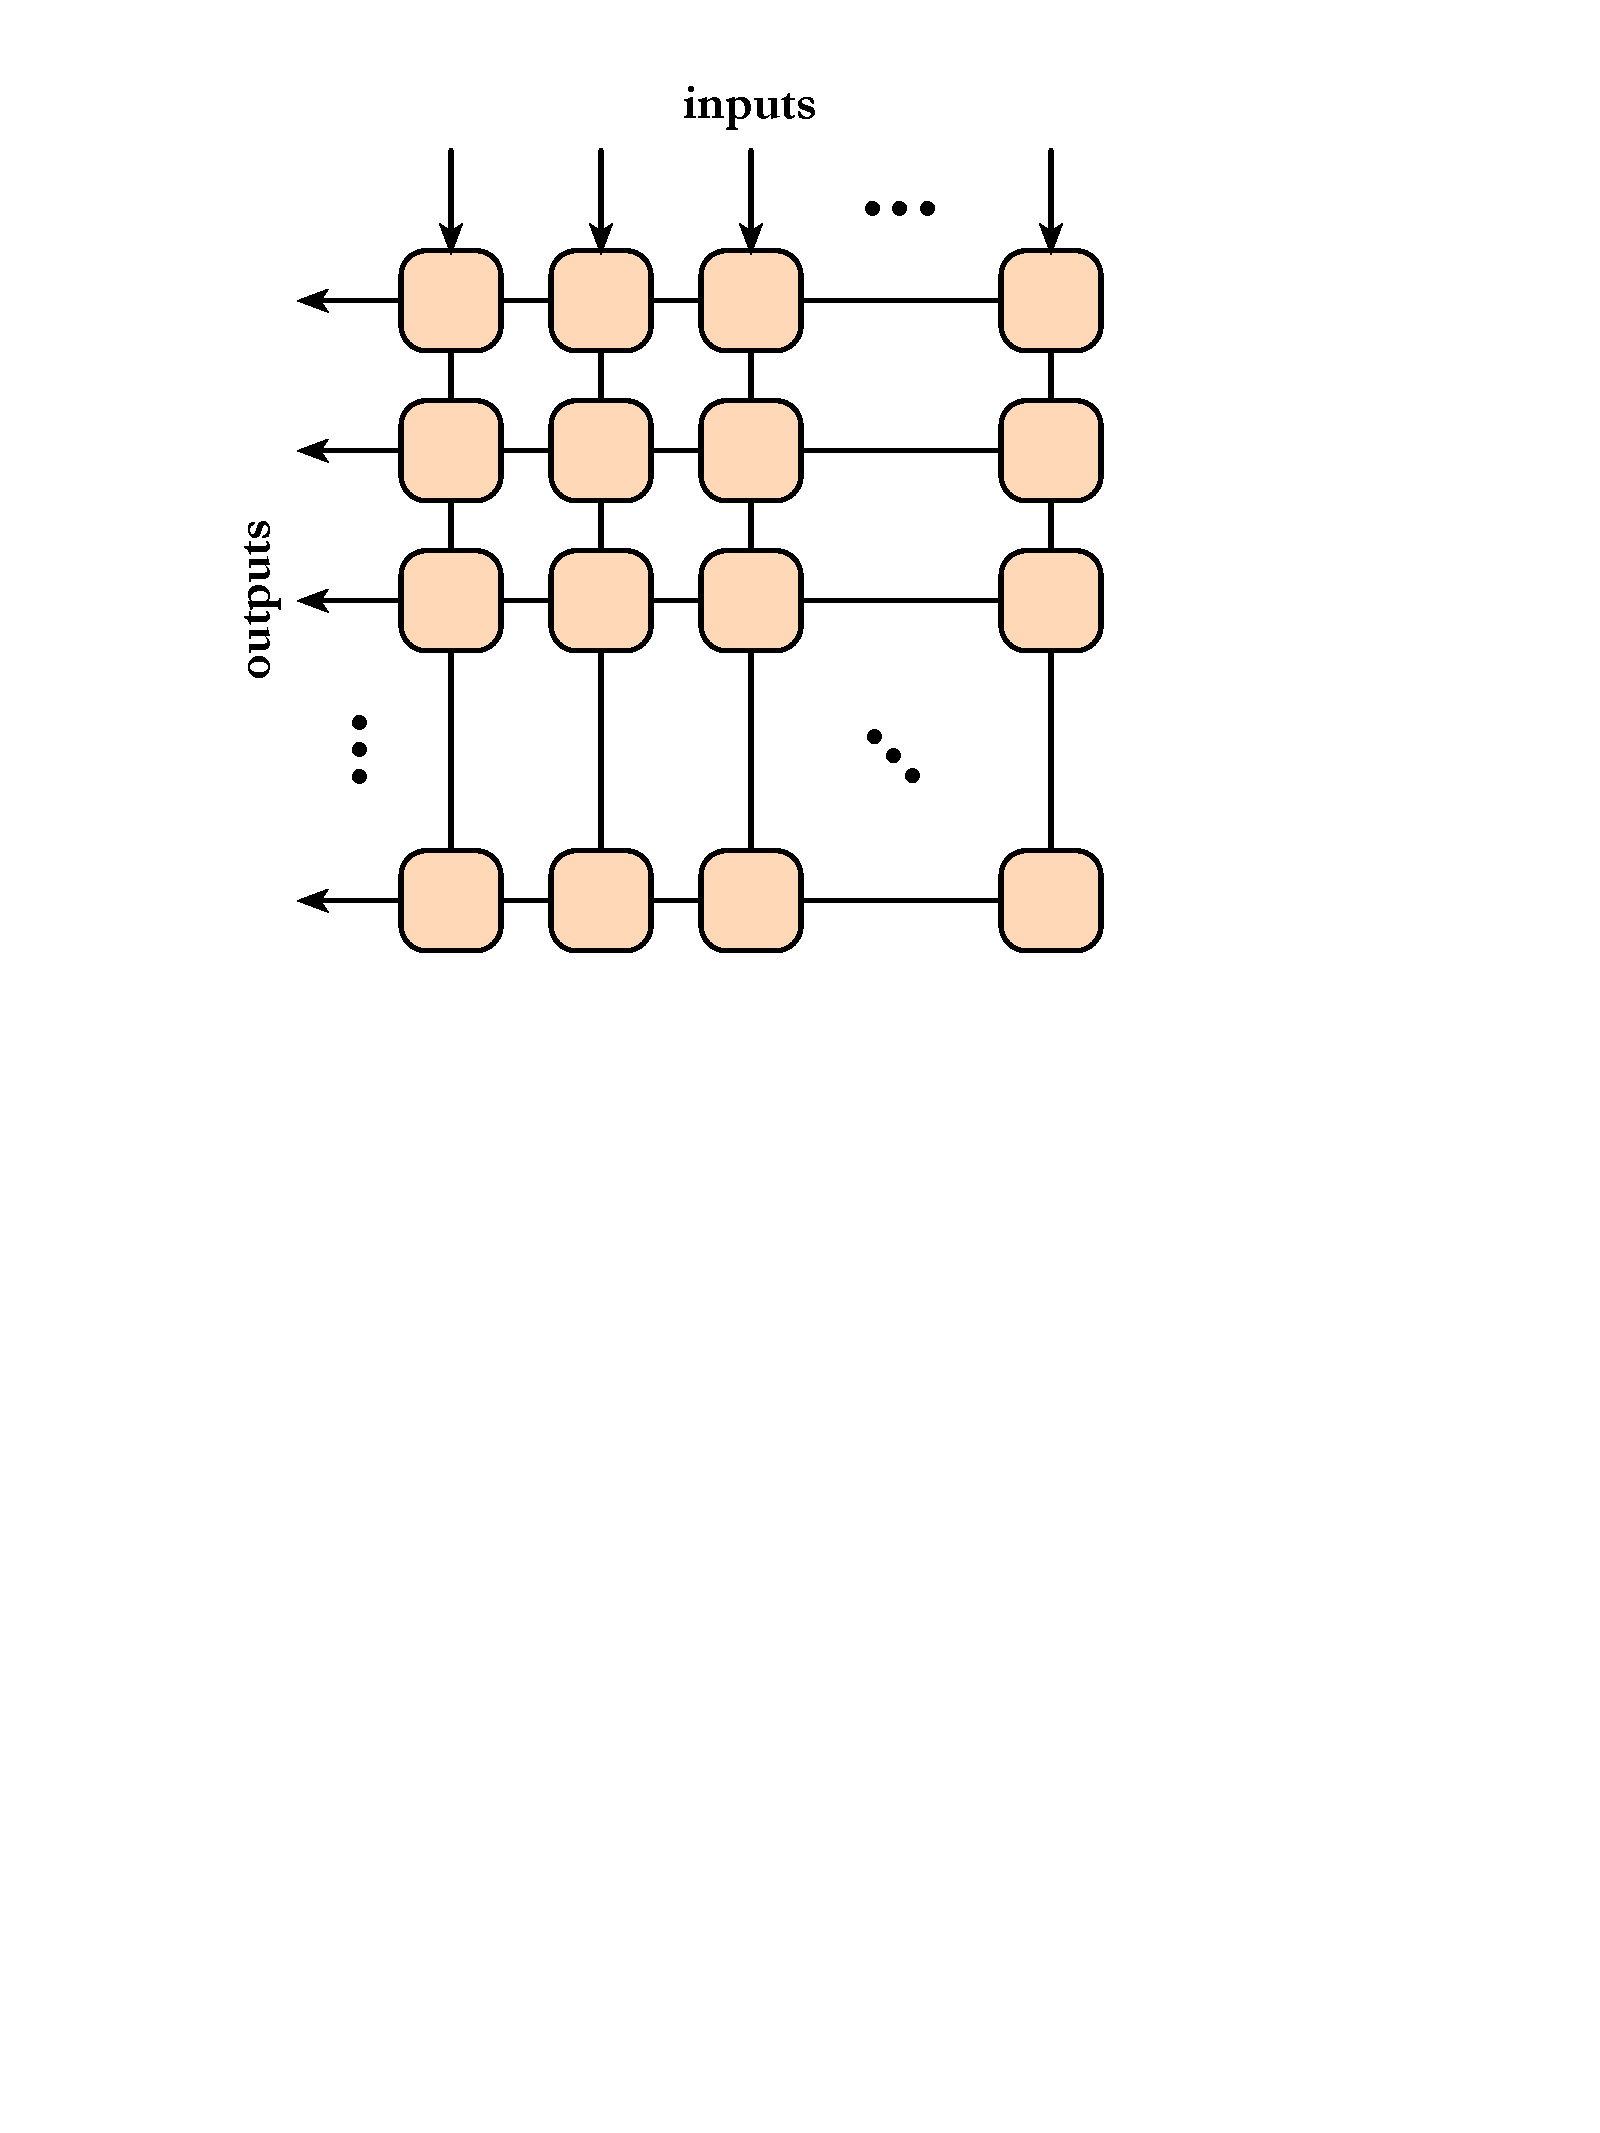
\includegraphics[clip=true, width=0.4\textwidth]{crossbar_switch}
\captionspacefig \caption{Crossbar architecture for multi-port switching. Each orange box represents a \mbox{$2\times 2$} switch, of any physical implementation. The switching sequence of the constituent two-port switches is defined by a binary \mbox{$n\times n$} permutation matrix, whose elements determine whether a given two-port switch flips modes or doesn't.} \label{fig:crossbar_switch}	
\end{figure}

\begin{figure}[!htbp]
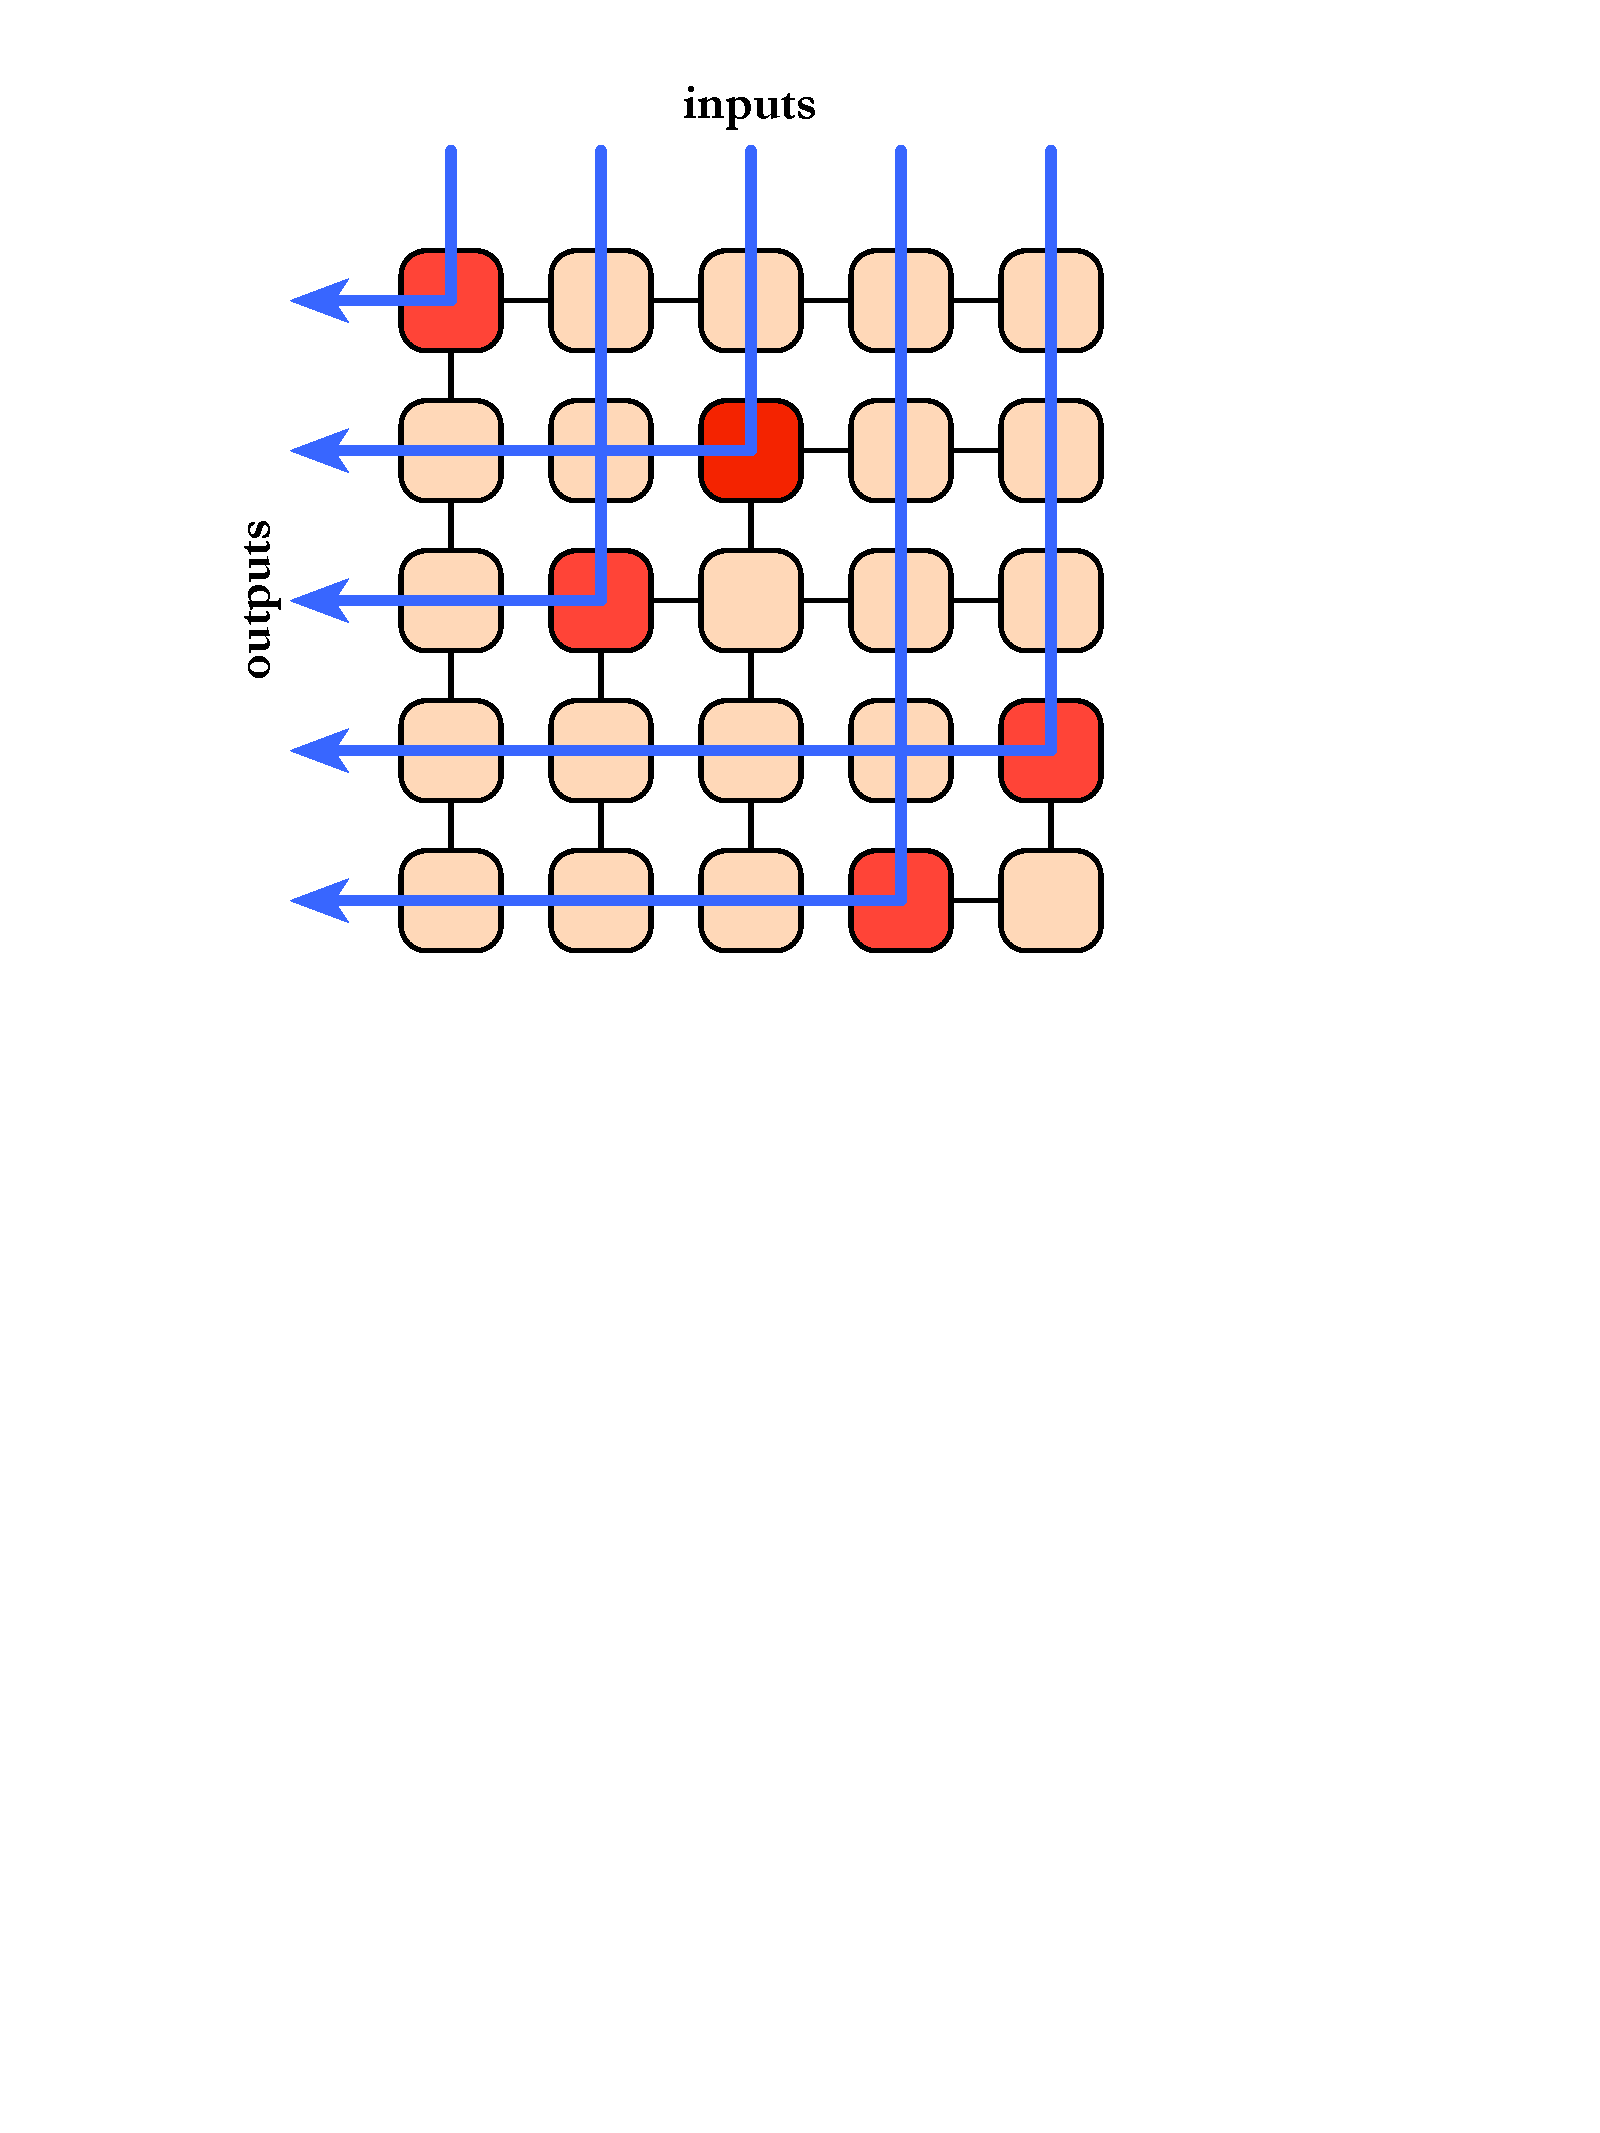
\includegraphics[clip=true, width=0.4\textwidth]{crossbar_example}
\captionspacefig \caption{Example switching configuration for a \mbox{$5\times 5$} crossbar switch. The switch colours represent whether the respective \mbox{$2\times 2$} switch is set to flip (red) the modes or not (orange).} \label{fig:crossbar_example}	
\end{figure}

Clearly the scheme requires $n^2$ two-port switches to implement arbitrary \mbox{$n\times n$} mode permutations. The main disadvantage of this scheme is that in general different paths within a given permutation experience differing optical depths, ranging from 1 (best case) to \mbox{$2n-1$} (worst case).